\documentclass[10pt,twocolumn,letterpaper]{article}

\usepackage{cvpr}
\usepackage{times}
\usepackage{epsfig}
\usepackage{graphicx}
\usepackage{amsmath}
\usepackage{amssymb}

% Include other packages here, before hyperref.

% If you comment hyperref and then uncomment it, you should delete
% egpaper.aux before re-running latex.  (Or just hit 'q' on the first latex
% run, let it finish, and you should be clear).
\usepackage[pagebackref=true,breaklinks=true,letterpaper=true,colorlinks,bookmarks=false]{hyperref}

\cvprfinalcopy % *** Uncomment this line for the final submission

\def\cvprPaperID{****} % *** Enter the CVPR Paper ID here
\def\httilde{\mbox{\tt\raisebox{-.5ex}{\symbol{126}}}}

% Pages are numbered in submission mode, and unnumbered in camera-ready
\ifcvprfinal\pagestyle{empty}\fi
\pagestyle{plain}
\begin{document}

%%%%%%%%% TITLE
\title{Project Report : Use Joint Embedding to Transform Food Image to Recipe}

\author{Sai Chen\\
Georgia Tech\\
{\tt\small schen721@gatech.edu}
% For a paper whose authors are all at the same institution,
% omit the following lines up until the closing ``}''.
% Additional authors and addresses can be added with ``\and'',
% just like the second author.
% To save space, use either the email address or home page, not both
\and
Ruiyang Li\\
Georgia Tech\\
{\tt\small rli386@gatech.edu}
\and
Shiya Song\\
Georgia Tech\\
{\tt\small ssong331@gatech.edu}
\and
Bing Yang\\
Georgia Tech\\
{\tt\small byang322@gatech.edu}
}

\maketitle
%\thispagestyle{empty}

%%%%%%%%% ABSTRACT
\begin{abstract}
   In this report, we utilized the published recipe1M+ dataset to study how to use deep learning models to understand food images.  We reimplemented the joint embedding model published in the recipe1M+ paper.  We changed and compared visual embedding models to study how visual models with varying levels of performance on classification problem can affect the performance on embedding estimation.  Our preliminary result showed that the quality of the joint embedding model can be improved by using better quality visualization model.
\end{abstract}

%%%%%%%%% BODY TEXT
\section{Introduction}

The recent success of applying deep learning methods for visualization tasks has truly proven the power of using ultra-large dataset for training complex models in human perception problems.  Despite the fast growing success in image classification and segmentation tasks, the problem of understanding the semantic meaning of images is still challenging for deep learning models.  One example studied in this project is described as follows: given a food image, generate the list of ingredients, the name of the dish, and a concise description of how to cook the food (cooking instructions).  The first task (namely classifying the ingredients) can be solved by combining object segmentation and classification tasks commonly used as benchmarks for visualization models.  However, generating cooking instructions requires information about aspects of the food ingredients other than their identities, the fact of which suggests that understanding the linguistic and semantic structure of the underlying recipe is important for the task of translating food images to recipes.

Due to the reasons described above, it is not surprising that previous existing work has focused on categorization of food images \cite{salvador2017learning} \cite{liu2016deepfood}.  Another problem with these approaches is that the they use medium-scale image datasets to train their models.  Considering the fact that performances on visualization tasks by deep learning models increase with larger and more complicated datasets, it is possible that the medium level performance of previous work (50.8\% in \cite{salvador2017learning}, 77.4\% in \cite{liu2016deepfood}, 79\% in \cite{7410503} and 80.9\% in \cite{ofli2017saki}) might be due to the limited size of the datasets utilized.

In 2017, Salvador et al \cite{salvador2017learning} recipe1M dataset, in which they collected and manually curated over 1 million food images and associated recipes for various downstream visualization tasks.  Subsequently in 2019, the same group improved the quality of the dataset by incorporating even more images and recipes in recipe1M+ \cite{marin2019learning}.  Briefly, the data collection process can be divided in two stages.  In the first stage, the authors downloaded over 1 million recipes and associated food images from popular websites for sharing recipes.  In the second the stage, the authors used every food image to search for more relevant images using an image search engine.  The result is the recipe1M/1M+ dataset.  The technical details for the data collection process can be found in \cite{marin2019learning}.

In this project, our goal is to utilize the recipe1M dataset to train a deep learning model that can be used to analyze the semantic meaning of food images with the help of the associated recipes.  Specifically, we are aiming at extracting useful representations of food images for downstream tasks, including categorization of food, translation to recipes and extract other useful information about the food, such as nutritional information.  We re-implemented the multi-modal join embedding model proposed in \cite{marin2019learning}.  In this model, representation of semantic meanings of a food image/its associated recipe are extracted by a visualization model/a modified LSTM model respectively.  The model is trained by minimizing the distance between the two representations (image/recipe text) in the join embedding space for pairs of images and recipes.  We specifically analyzed whether using different visualization models with varying performance on image classification tasks affect the performance on the current task.

Deep learning model that can extract semantic structures of food images has multiple applications.  First, automatic translation from food images to recipes can be useful for non-professional cooking education.  Second, this model can facilitate the automatic collection of information about food from social network websites.  Such information includes nutritional information in different countries or areas, approaches of food preparation in different cultural backgrounds and health condition for different populations.  Third, comparing different visualization models for generating embeddings can be used to help improve the quality of the information retrieval process.

Below we will discuss the details of our implemented model.  We will also talk about how we train our model and present results on the performance of our model.

%-------------------------------------------------------------------------
%------------------------------------------------------------------------
\section{Approach}

\subsection{Data preparation}
We downloaded our data from \href{http://im2recipe.csail.mit.edu/dataset/download/}{recipe1M website}.  There are three components in the downloaded dataset: images, recipe text and pretrained data.  We preprocessed the data by borrowing/modifying the \href{https://github.com/torralba-lab/im2recipe-Pytorch}{github repo} provided by the author for downstream training.  More specifically, we created a LMDB database for loading data during training.  Each data entry in the database contains the following components: the file path of the a food image, the pre-trained embeddings for ingredients and cooking instructions for the associated recipe (details discussed in the model section) and the food category defined in Fodd-101 dataset \cite{bossard14}.  The partition of the data entry (train/validation/test) is pre-defined by the database creator and we follow their partition in our training process.

During data preparation, we found out that the size of the dataset is too large to be processed following the original code repo.  We made modifications to the \href{https://github.com/torralba-lab/im2recipe-Pytorch}{github repo} so that we can build all three LMDB datasets (train/validation/test) separately and in the limited amount of storage on google drive.  We shared data using google drive and used google colaboratory for all downstream processing.

\subsection{Model}
All codes used for the following analysis are either directly borrowed from or modified based on \href{https://github.com/torralba-lab/im2recipe-Pytorch}{this github repo}.  The model we used in this project for the embedding extraction task is the same as \cite{marin2019learning} and is illustrated in Figure \ref{fig:f1}.  The general principle of this model is to match the embedding extracted from a food image to the embedding extracted from the associated food recipe.  There are two major components in this model: a Convolutional Neural Network (CNN) to extract image embedding and a multi-component LSTM to extract text embedding.

\subsubsection{Image Embedding}
To extract image embedding, we utilized pre-trained CNN for image classification task from pytorch models module.  The last fully connected layer to generate the class probabilities is removed to retain the features extracted in the second-to-last layer.

In this project, our main goal is to compare how different visualization models with varying performance on classification tasks can affect the joint embedding model.  We choose to use VGG-19, ResNet-18 and ResNet-50 for downstream comparisons.  These three models differ in their model complexity and performance on ImageNet classification dataset, and are commonly used as baseline for method development.

\subsubsection{Text Embedding}
The process of extracting embedding from recipe texts are divided into two stages.  In the first stage, recipe text are divided into two parts: ingredients and instructions.  Ingredients of a food recipe were extracted using bigrams and were converted to standard names using nutrient database from United States Department of Agriculture (USDA).  Once ingredient lists for all recipes are standardized, a word2vec model was trained on this dataset to extract the embeddings for ingredients alone.  For instructions, the authors used skip-thoughts method \cite{NIPS2015_f442d33f} to model the context of instructions in a single recipe.  The result is a extracted representation for each instruction in a series of instructions for a single food recipe.  The trained ingredients embeddings and skip-thought vectors for instructions can be downloaded from \href{http://im2recipe.csail.mit.edu/dataset/download/}{recipe1M website}.  To focus on the joint embedding model itself, we decided to download and use the pre-trained embeddings in the recipe text part.  These embedding data for both ingredients and instructions are stored in the LMDB database discussed in the Data Preparation section.

In the second stage, the embeddings for ingredients and instructions trained by using corpus of text data are used as inputs to learn a combined embeddings from the recipe text (illustrated in Figure \ref{fig:f1}).  Following the original paper, we used a bi-directional LSTM to extract embedding from ingredients and a single layer LSTM to extract embeddings from skip-thought vectors for instructions.  We combined these two embeddings using a single linear layer so that the resulted embedding has the same dimension as the image embedding.  For both LSTM encoders, the input is a sequence of learned embeddings from the first stage discussed above.

\subsection{Loss Function}
We used cosine similarity with margin as the loss function during training.  The cosine similarity is defined as
\[
\small
L(e_i, e_t, y) = 
\begin{cases}
	1 - cos(e_i, e_t), & \text{if } y = 1 \\
	max(0, cos(e_i, e_t) - \alpha), & \text{if } y = -1
\end{cases}
\]

, in which \(e_i\) is the embedding for image and \(e_t\) is the embedding for the text.  When loading samples from the database, there are 20\% chance that the loaded pair of food image and recipe match with each other.  In the remaining 80\% cases, a random recipe is selected from the database to pair with the loaded food image in order to train the cosine similarity loss.

The author of the recipe1M paper adds another layer of optimization goal to further improve the performance of the learned embeddings.  Specifically, we used Food-101k and bigrams of recipe titles to generate a class label of each food image/recipe, namely what the food is called in English.  When train the joint embedding model, another objective was added to the optimization problem: the learned embeddings from both food images and recipe texts should accurately predict the food class they are given.  Mathematically, the final loss function becomes:
\[
\small
L(e_i, e_t, c_i, c_t, y) = L_{cos}(e_i, e_t, y) + {\lambda}L_{class}(e_i, e_t, c_i, c_t)
\]
in which \(L_{cos}\) is the cosine similarity loss, \(L_{class}\) is the cross-entropy loss associated with classifying the right food category, \(c_i\) is the food category assigned to the image and \(c_t\) is the food category assigned to the recipe text.  \(\lambda\) is the weight parameter used to adjust the relative importance of the two loss functions and is set to 0.02 following the original paper.

\subsection{Implementation}
We implemented our model in pytorch (version 1.10, python = 3.9).  All hyper-parameters are copied from the original paper.


\section{Experiments and Results}

\subsection{Experiment Setup}
We implemented the above mentioned joint embedding model in PyTorch.  To study how visualization models with varying performance on classification problems can affect the join embedding model, we implemented three versions with different pre-trained image models from torchvision module in pytorch: VGG-19 with batch normalization (BN), ResNet-18 and ResNet-50.  The ResNet-50 model is the original model used in the recipe1M paper.  We chose VGG-19 with batch normalization because it is among the earliest proposed image models and has a descent performance on ImageNet 1-crop dataset.  We chose ResNet-18 to compare models with similar network design but different complexities and power.  The order of accuracy@5 for these models on ImageNet 1-crop dataset can be checked at \href{https://pytorch.org/vision/stable/models.html}{torchvision website} and are listed here for reference: 91.842\% for VGG-19 with BN, 89.078\% for ResNet-18 and 96.862\% for ResNet-50.

All data are pre-partitioned into train, validation and test within the downloaded dataset.  In total, there are 619,508 training images, 133,860 validation images and 134,338 test images.

\begin{table*}
\begin{center}
\begin{tabular}{|l|c|p{8cm}|}
\hline
Hyperparameters & Value \\
\hline\hline
Mismatch rate & 0.8 \\
Learning rate & 0.0001 \\
Regularization weight & 0.01 \\
Number of epochs & 100 \\
Early stop & 1000 \\
Batch size & 16 \\
Number of Random samples for calculating median rank & 1000 \\
\hline
\end{tabular}
\end{center}
\caption{Hyperparameters in this project}
\label{tab:hyperparams}
\end{table*}

All the hyper-parameters are collected from the original paper and are listed in Table \ref{tab:hyperparams}.  To use the cosine similarity loss, we generated the dataloader so that the food image and the recipe in 80\% of the samples are mismatched and the remaining 20\% are matched.  In the original paper, the authors mentioned that the model converged at ~300 epochs with all training data in ~3 days.  When we started running the model, we found out that it took ~50 hours to finish running a single epoch.  The main problem is that we transferred all our data to google drive for training using the google colab service.  Data transfer from mounted google drive disk to the disk of the runtime virtual machine in google colab takes unreasonably amount of time.  We suspect that this is due to the approach used for transferring data between the two using network connections instead of memory to cpu.  One way to solve this is to copy all data to the disk of the runtime virtual machine.  However, the size of the whole dataset (~300 GB) is too large to fit into the space google colab can provide.  Thus, we decided to stop each epoch early (1000 batches) so that the running time is reasonable for this project.  This approach is equivalent to running through the whole dataset ~2.5 times (\(\frac{1000 batches * 16 samples/batch * 100 epochs}{~600,000 samples}\)).  Another roadblock we encountered when using Google Colab runtime is that colab offers limited time for background execution.  That is, Colab will forcefully disconnect user runtime after an arbitrary amount of time. Although the Colab Pro subscription increased the cap for that, we were still given only from 3-hours to 10-hours for each session. This further limited the number of examples that we can use to train the models. 

We fully realized that this approach can make the training process unstable and inefficient, as can be seen from the result section.  However, we do believe that by training different models using the same setup, we can compare the performance of different models in a fair manner.

We chose the optimizer based on the original paper.  We used Adam optimizer with learning rate set to 0.0001.  We did try different learning rate on the ResNet-50 model and found out that the training process became even more unstable.  Validation is performed every 5 epochs.  Following the original paper, we trained parameters from either visualization model and text model in alternating stages to avoid any complexity caused by mixed training.  Specifically, when the validation metric keeps getting worse for more than 3 times, we switch training from parameters of one part (visual/text) to the other part (text/visual).  We found out this approach helps to get out of local minimum.

Since we utilized the skip-thought vectors provided by the authors, it is impossible to convert food images to recipes without knowing the architecture of the encoder used to generate those vectors.  In order to evaluate and compare our models in a meaningful way, we decided to use the median rank and recalls as our performance metrics.  Median rank is calculated as follows.  During each validation stage, we randomly select 1,000 pairs of (image embedding, text embedding) after running the model through all selected validation samples.  We compute the similarity matrix between all selected image embeddings and text embeddings.  For each image, we then find out the rank of its corresponding recipe in the similarity matrix.  We take the median of ranks across all images and return the average value of this median after 10 replications.  Median rank is used to evaluate how good the embeddings generated by our encoder for food image match with the underlying recipes across a random pool of recipes.  Using the same similarity matrix, we compute the percentage of images that have their matching recipes ranked in top 1, 5 and 10 positions across all selected recipes.  Below, we will use cosine similarity loss to track the training progress, and use median rank to track the performance evaluated in validation phase during training.  We will also show and compare the performance of the three models on the test dataset.

\subsection{Results}
As discussed above, due to the limit in resources, we can only run 100 epochs of training, with 1,000 batches each containing 16 training samples in each epoch.  We run validation every 5 epochs.  Figure \ref{fig:f2} shows our results.  As expected, with the limited amount of data used for training during each epoch, the cosine similarity loss does not change much for all three different models.  The training curves in all three cases are flat.  However, we did observe that on the validation dataset, the model with the best performance on ImageNet, namely the ResNet-50, had the best performance at the end.  In over 1,000 random samples, the matching recipe ranked on average ~42 for a food image.  Surprisingly, other two models showed decreased performance over training.  Another unexpected observation is that in the validation curve for the ResNet-50 model, there are two spikes showing decreased performance (increased median rank).  The target of the optimizer transitioned from parameters of text to that of image after the first spike, and changed in the other direction after the second spike.  Overall, the ResNet-50 model has the best performance, as can also be seen from test in Table \ref{tab:perfontest} using the best trained model from all 3 settings.

We thought that the decrease in validation performance might be due to one possible reason.  We noticed that all the hyperparameters used in the original paper are tuned towards using ResNet-50 as the visualization model.  It is very likely that these hyper-parameters, including learning rate and batch size, are not suitable for the other two models.  This problem might even get worse in our experiment, since we used early stopping to limit the amount of data used in each epoch, which creates a strong bottleneck in data usage during training.  However, due to the limit of time in this project, we won't be able to fully explore this possibility with enough parameter tuning.  But this can be one possible future direction for the current project.

Even with restricted data usage, our results showed that the model with the best performance on classification task also performs the best in the join embedding model.  This result suggests that using a high-quality model in transfer learning for downstream tasks can help improve the quality of the overall model.

\begin{table*}
\begin{center}
\begin{tabular}{|l|c|c|c|c|}
\hline
Dataset & Median Rank & Recall at 1 & Recall at 5 & Recall at 10 \\
\hline\hline
VGG-19 with BN & 81.2 & 0.009 & 0.045 & 0.086 \\
ResNet-18 & 125.4 & 0.004 & 0.0183 & 0.045 \\
ResNet-50 & 45.3 & 0.029 & 0.103 & 0.154 \\
\hline
\end{tabular}
\end{center}
\caption{Performance on the test dataset (best model, after first 5 epochs)}
\label{tab:perfontest}
\end{table*}

\section{Conclusion and Future Directions}

Based on the results presented above, the immediate next step is to confirm why our implementation is not able to replicate the paper, more specifically, why the training loss is almost flat in ResNet-50, and why both training and validation performance decrease for VGG-19 and RestNet-18. 

As mentioned in the previous session, the total number of training samples we used is only equivalent to ~2.5 epochs in the original paper. The number of training data we presented to the model is far less than the amount needed for convergence. Our plan is to increase the number of epochs and batch size in another computing platform to achieve better performance.

As discussed in the result section, we hypothesized that the hyperparameters used in our project might not be optimal for ResNet-18 and VGG-19 BN.  To solve this issue, we will tune the model with other sets of hyperparameters and learning rate decay modules. 

For the mysteriously decreasing performance in the validation dataset at the beginning of the training, our hypothesis is as follows. Note that for the pre-trained visualization models, the training labels include wider range of categories other than food. For example, in pre-trained ResNet models \cite{he2015deep}, categories for food only constitutes a small portion of the training dataset. The high-level features extracted in those models may not represent properties of cooked food useful for our defined task. Because all food101k classes are sub-categories of cooked food, there might be class imbalance in the initial epochs during transfer learning.   Because of that, all input images are located close to each other in the feature space learned by the visualization models. While the training moves on and the extracted features can capture more and more food specific characteristics, we should observe a more balances output class. To confirm this hypothesis, after each training epoch, we are going to connect the output features from the visual model to its original last feed forward layer to monitor the density distribution of the output class.

Another part of the model that can potentially be improved is the cosine embedding similarity loss function used for the optimizer. The original loss function optimized cosine embedding similarity loss function to one (zero-degree difference between the direction of embeddings) when the food image class matches the recipe, while it tries to optimize the loss function to zero (ninety-degree difference between the direction of embeddings) when the image and recipe do not match.  We think there could be space for improvement for the loss function.  Conceptually, the similarity may not need to be optimized to zero for different classes, e.g., the difference between roasted chicken and fried chicken might be smaller than the difference between roasted chicken and ice cream. We plan to add another term in the loss function that represent the cosine embedding similarity in the input word-embedding to change the point we optimized to when image class and description class is different.

Lastly, the joint embedding model can help use further understand the meaning of high-level features extracted in the visualization modules. We can use this scheme to train a simple discriminator and change specific parts in the recipe (for example, cooking style) to see how the extracted visulization embeddings change. This can help us further understand the semantic meaning of a high-level features extracted in visualization module.

\section{Work Division}

Contributions of each group member can be found in Table \ref{tab:contributions}.

\begin{table*}
\begin{center}
\begin{tabular}{|l|c|p{8cm}|}
\hline
Student Name & Contributed Aspects & Details \\
\hline\hline

Sai Chen & Data Creation and Implementation & 
Download, extract and transfer data to the shared google drive. \newline\newline
Implement the model for ResNet-50 \newline
\emph{recipe\_model\_resnet50.py}. \newline\newline
Train the model with ResNet-50 module. \newline
\emph{train\_resnet50.py}, \emph{notebook\_resnet50.ipynb} \newline\newline
Create the plot\newline
\emph{cs7463-plot-result.ipynb} \newline \\
\hline

Ruiyang Li & Implementation and Report & 
Implement the model for ResNet-18 \newline
\emph{recipe\_model\_resnet18.py}. \newline\newline
Train the model with ResNet-18 module. \newline
\emph{train\_resnet18.py}, \emph{notebook\_resnet18.ipynb} \newline\newline
Write the discussion section of the report. \newline \\
\hline

Shiya Song & Implementation and Report & 
Implement the model for VGG-19 with BN \newline
\emph{recipe\_model\_vgg.py}. \newline\newline
Train the model with ResNet-50 module. \newline
\emph{train\_vgg.py}, \emph{notebook\_vgg.ipynb} \newline\newline
Write the result section of the report. \newline \\
\hline

Bing Yang & Proposal, Base Implementation and Report & 
Write the proposal. \newline\newline
Rewrite the scripts for data preparation following the recipe1M base code. \newline
\emph{get\_vocab.py, mk\_dataset.py, bigrams.py, utils.py, proc.py} \newline\newline
Write the base code for training models. \newline
\emph{params.py, data\_loader.py, recipe\_model.py, train.py, test.py} \newline\newline
Write the introduction and method sections of the paper. \newline \\
\hline
\end{tabular}
\end{center}
\caption{Contributions of team members.}
\label{tab:contributions}
\end{table*}




%-------------------------------------------------------------------------


\begin{figure*}[t]
\begin{center}
\fbox{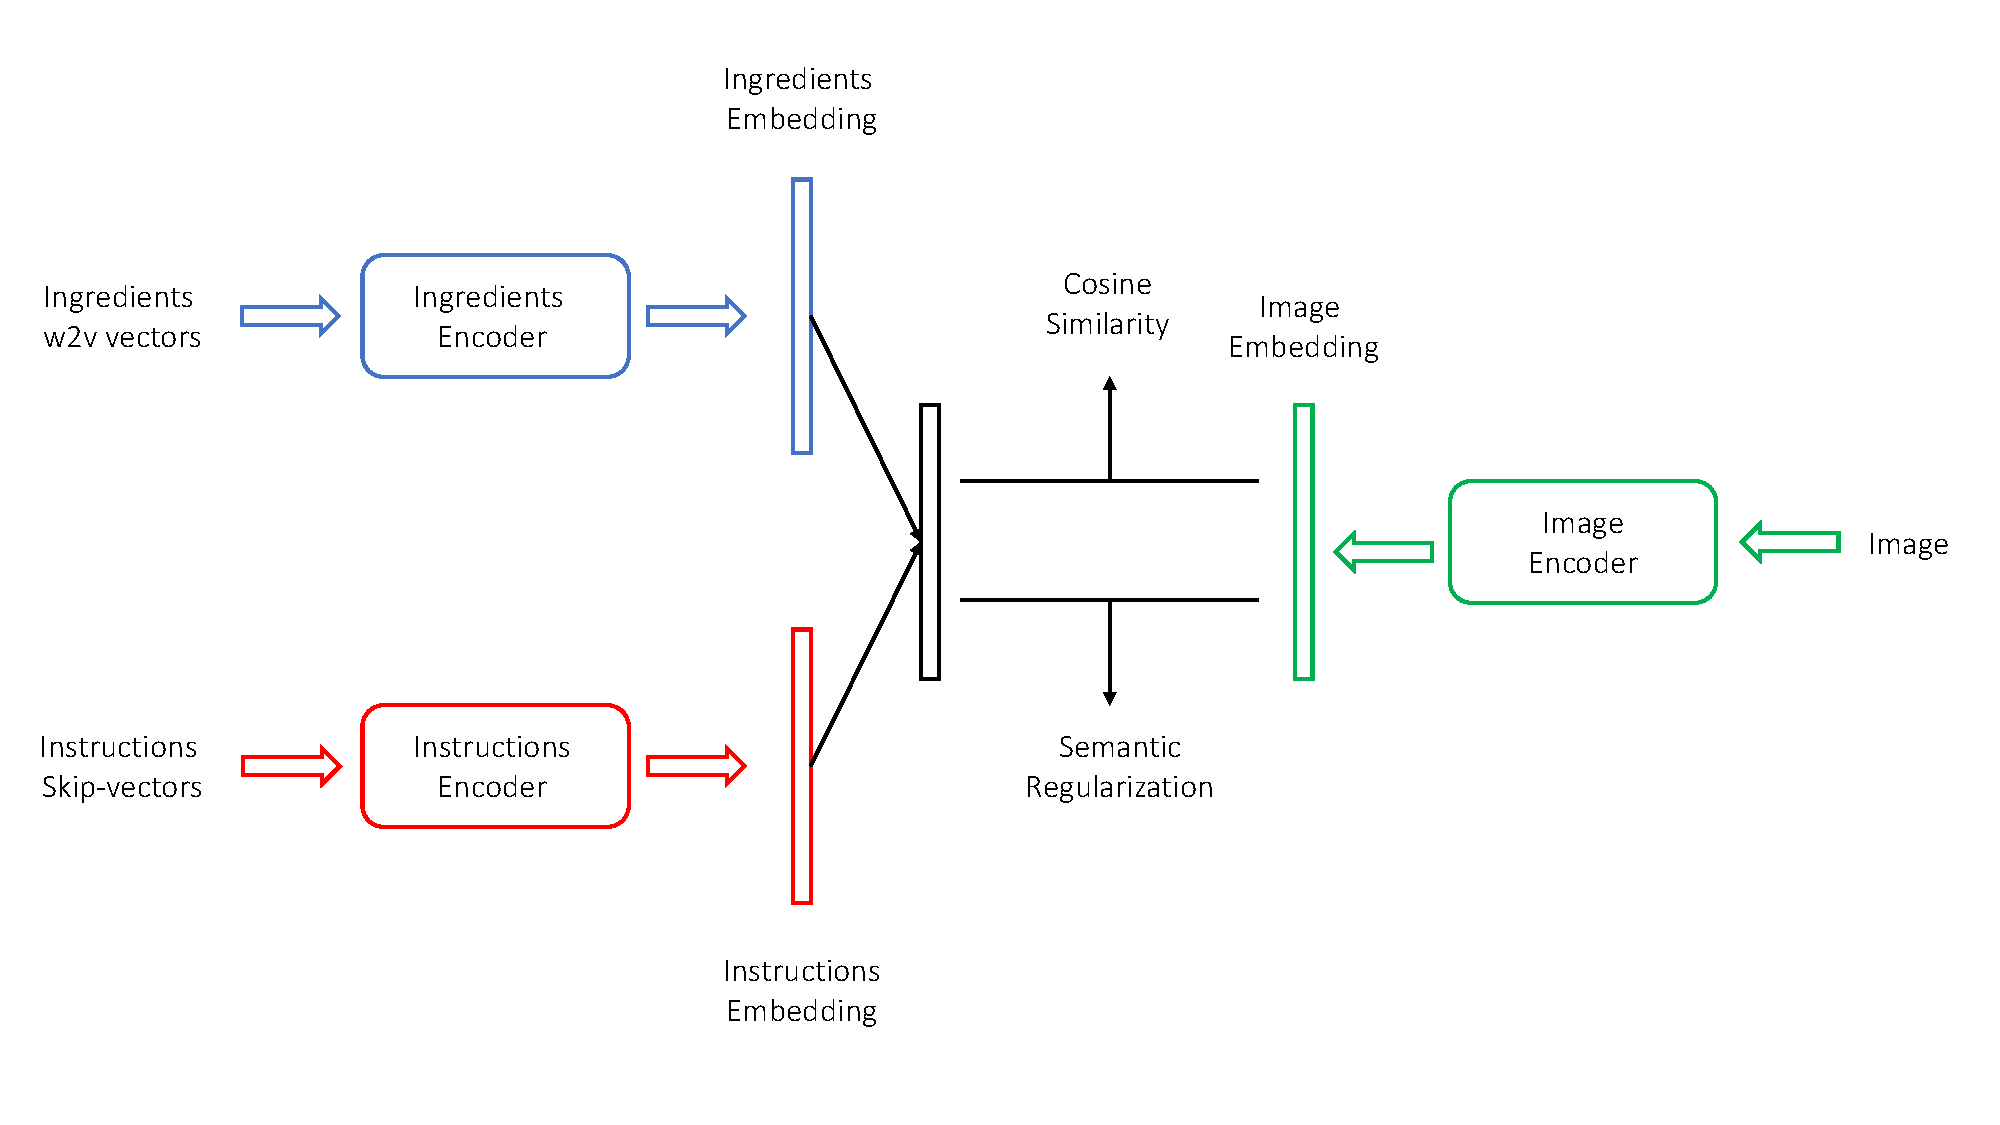
\includegraphics[width=1.0\linewidth]{Figure1.pdf}}
\end{center}
   \caption{Illustration of the model. Recreated from Marin et al, 2019}
\label{fig:f1}
\end{figure*}

\begin{figure*}[t]
\begin{center}
\fbox{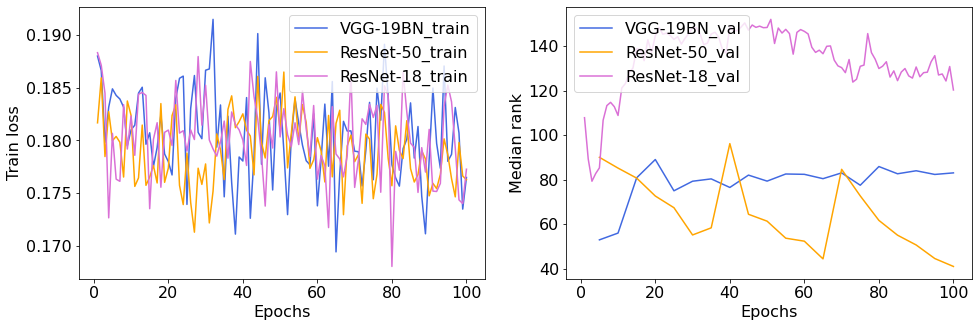
\includegraphics[width=1.0\linewidth]{train_val_loss.png}}
\end{center}
   \caption{Training loss and validation median rank}
\label{fig:f2}
\end{figure*}




%-------------------------------------------------------------------------




{\small
\bibliographystyle{unsrt}
\bibliography{CS7643-Report}
}

\end{document}
